% Provenance (never printed): enseignement scientifique premiere (2019),
% "Le Soleil, notre source d'energie" (power received by latitude and
% season, albedo, the Earth's radiative balance, the small share stored by
% photosynthesis) and the old seconde/premiere S material on the
% atmosphere's energy; see sources/book2/PROVENANCE.md. Every insolation
% value, budget closure and photosynthesis figure is computed in
% figdata/grade-10/energy_budget.py; the budget fluxes are AR6 WG1
% Figure 7.2.
\chapter{De energiebalans van de Aarde}\label{ch:g10:earth-energy-budget}

Op de langste dag van het jaar gaat de Zon op de Noordpool niet onder. Ze
draait de hele dag op dezelfde hoogte, ongeveer \qty{23}{\degree} boven de
horizon, rond aan de hemel, en de top van de atmosfeer boven de pool ontvangt
op één dag meer zonlicht per vierkante meter dan waar ook op Aarde ---
\qty{13.0}{kWh}, tegen \qty{9.5}{kWh} boven de evenaar. Toch blijft de zee rond
de pool de hele zomer met ijs bedekt. Over een heel jaar gerekend ontvangt de
evenaar daarentegen twee en een half keer zoveel zonlicht als de pool, en
blijven de tropen het hele jaar warm. Dit hoofdstuk volgt de energie van het
zonlicht: hoeveel er aankomt, waar en wanneer; hoeveel er meteen naar de ruimte
wordt teruggekaatst; hoe de rest verdeeld wordt tussen de lucht en de grond,
van de tropen naar de polen wordt gevoerd en ten slotte als infrarood licht
naar de ruimte teruggaat --- en welk piepklein deel ervan door levende wezens
wordt opgeslagen.
% ledger: earth:TSI, earth:obliquity (daily totals computed in figdata/grade-10/energy_budget.py)

\begin{omfigure}
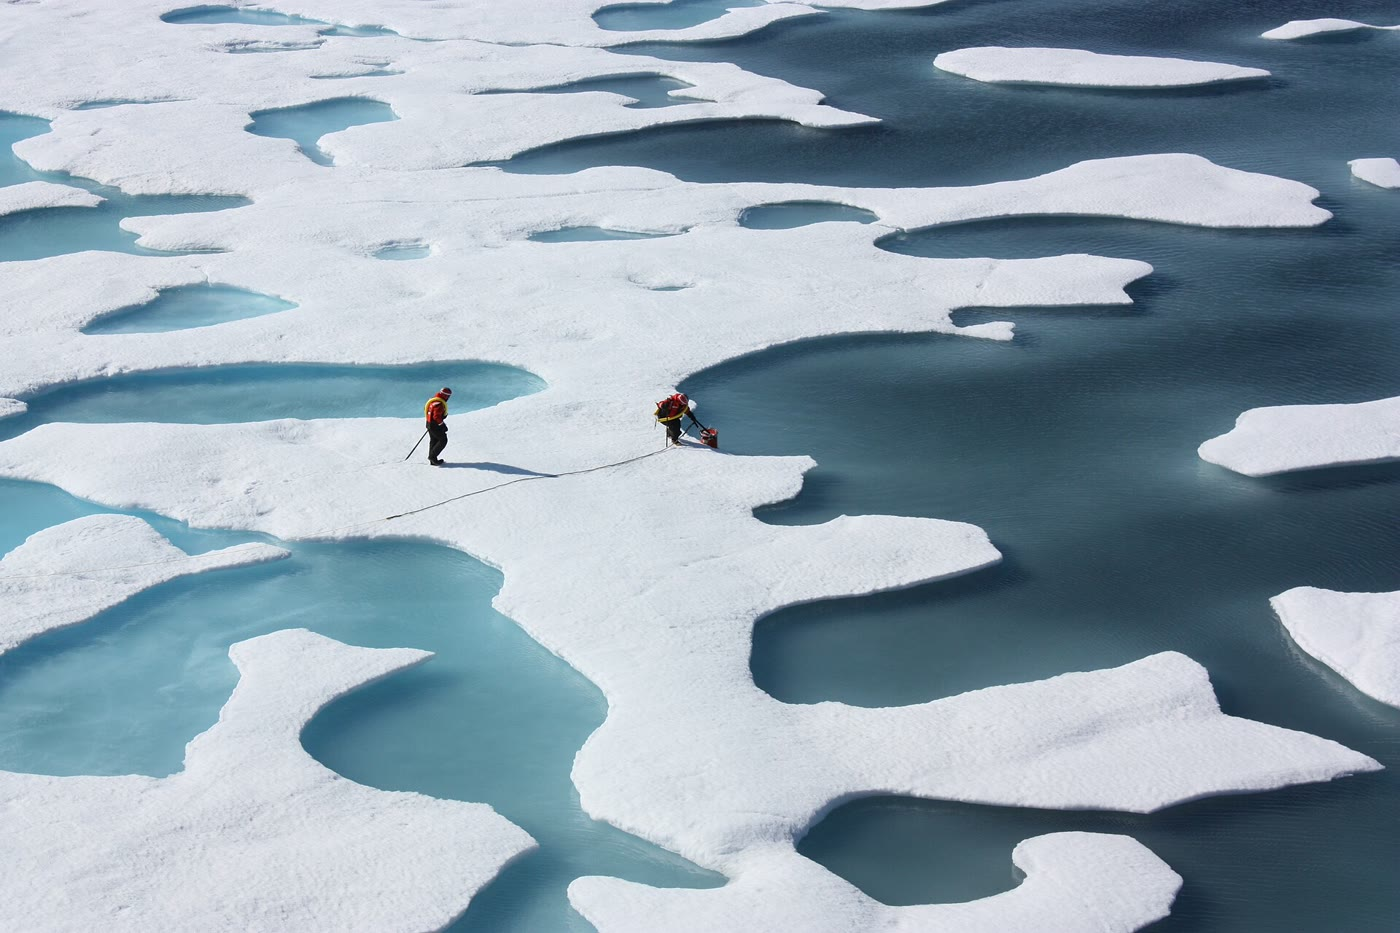
\includegraphics[width=0.78\linewidth]{images/book2/g10-nasa-melt-ponds.jpg}

{\small Zee-ijs in de Noordelijke IJszee in juli, onder een Zon die niet
ondergaat: wit ijs, plassen smeltwater op het oppervlak, en de donkere open zee
tussen de ijsschotsen. Twee wetenschappers nemen monsters van de plassen. Foto:
NASA Goddard Space Flight Center, 2011 (publiek domein).}
\end{omfigure}

\begin{recall}
De seizoenen ontstaan door de helling van de aardas, \qty{23.44}{\degree} ten
opzichte van de loodlijn op het vlak van haar baan: in juni helt het noordelijk
halfrond naar de Zon toe, die daar hoger aan de hemel klimt en langer
boven de horizon blijft (de natuurkundeboeken en Boek 1). De
bestralingssterkte op de afstand van de Aarde, $S_0 = \qty{1361}{W/m^2}$, het
bondalbedo van een planeet en haar \omterm{def:g10:habitable-planet:equilibrium-temperature}{evenwichtstemperatuur} kwamen aan bod in
\cref{ch:g10:habitable-planet}. Broeikasgassen absorberen een deel van het
infrarood dat het oppervlak uitzendt (de scheikundeboeken). Warme lucht stijgt
op en koude lucht daalt; zo gaat de lucht rond in convectiecellen en ontstaan
de wereldwijde winden (Boek 1, jaar 8). Planten, algen en sommige bacteriën
maken met de energie van licht suikers uit koolstofdioxide en water:
fotosynthese (de biologieboeken).
\end{recall}

\section{Het ontvangen zonlicht}

Vanaf de Zon gezien is de Aarde een schijf. Elke seconde vangt ze het zonlicht
op dat op een schijf met straal $R$, haar eigen straal, valt; maar dat licht
wordt verdeeld over alle punten van een bol, waarvan de helft in de nacht ligt.

\begin{proposition}[Een kwart van de zonneconstante]\label{prop:g10:earth-energy-budget:quarter}
Gemiddeld over het hele aardoppervlak en over dag en nacht is het vermogen van
het zonlicht dat aan de top van de atmosfeer aankomt
\[
  \frac{S_0}{4} = \frac{1361}{4} \approx \qty{340}{W/m^2}.
\]
\end{proposition}

\begin{proof}
De Aarde vangt het zonlicht op dat door een schijf met oppervlakte $\pi R^2$
loodrecht op de stralen gaat, dus een vermogen $S_0\,\pi R^2$. Verdeeld over de
oppervlakte van de bol, $4\pi R^2$, geeft dat $S_0\,\pi R^2/(4\pi R^2) =
S_0/4$ per vierkante meter.
\end{proof}
% ledger: earth:TSI, ipcc:budget-toa

\begin{omfigure}
\begin{tikzpicture}[font=\small, >={Stealth[length=2mm]}]
  \foreach \y in {-1.2,-0.8,...,1.21}
    \draw[->, omProp!80!black] (-3.4,\y) -- (-1.75,\y);
  \node[anchor=south, font=\footnotesize, align=center] at (-2.6,1.35) {zonlicht,\\$S_0$ per m$^2$};
  \draw[fill=omProp!15, draw=omProp!80!black] (-1.6,0) ellipse (0.18 and 1.3);
  \node[anchor=north, font=\footnotesize, align=center] at (-1.6,-1.4) {schijf\\$\pi R^2$};
  \shade[ball color=omDef!35] (1.2,0) circle (1.3);
  \fill[black, opacity=0.35] (1.2,1.3) arc (90:-90:1.3) arc (-90:90:0.35 and 1.3);
  \draw[omDef!80!black] (1.2,0) circle (1.3);
  \draw[dashed, black!50] (1.2,-1.3) arc (-90:90:0.35 and 1.3);
  \draw[<->] (1.2,0) -- node[above, font=\footnotesize] {$R$} (2.5,0);
  \node[anchor=west, font=\footnotesize, align=left] at (2.8,0.7) {bol $4\pi R^2$:\\half in het daglicht,\\half in de nacht};
  \node[anchor=west, font=\footnotesize, align=left] at (2.8,-0.75) {gemiddeld:\\$S_0\pi R^2/4\pi R^2 = S_0/4$};
\end{tikzpicture}

{\small De Aarde vangt het zonlicht op dat op een schijf met haar eigen straal
valt, maar verdeelt het over de vier keer grotere oppervlakte van een bol:
gemiddeld ontvangt elke vierkante meter van de top van de atmosfeer een kwart
van de zonneconstante.}
\end{omfigure}

Het gemiddelde verbergt grote verschillen van plaats tot plaats. Een bundel
zonlicht die schuin op de grond valt, verspreidt zich over een grotere
oppervlakte dan een bundel die er loodrecht op valt.

\begin{proposition}[Zonlicht op een horizontaal oppervlak]\label{prop:g10:earth-energy-budget:height}
Staat de Zon op een hoogte $h$ boven de horizon, dan ontvangt een horizontale
vierkante meter aan de top van de atmosfeer het vermogen $S_0 \sin h$.
\end{proposition}

\begin{proof}
Neem een vierkante bundel zonlicht met een doorsnede van \qty{1}{m^2}, die
$S_0$ draagt. Op de grond is zijn voetafdruk een rechthoek met één zijde van
\qty{1}{m} en een andere met lengte $\ell$ in de richting van de schuine
stralen. In de rechthoekige driehoek gevormd door die zijde, de straal en de
doorsnede van de bundel is de hoek bij de grond $h$ en geldt $\sin h = 1/\ell$.
Het vermogen van de bundel wordt over $\ell$ vierkante meter verdeeld:
$S_0/\ell = S_0 \sin h$ per vierkante meter.
\end{proof}

\begin{omfigure}
\begin{tikzpicture}[font=\small, >={Stealth[length=2mm]}]
  \fill[omExo!15] (-0.3,-0.5) rectangle (6.3,0);
  \draw[thick] (-0.3,0) -- (6.3,0);
  \foreach \s in {0,0.3,...,1.21}
    \draw[->, omProp!80!black] ({0.6+\s/sin(35)+3.2*cos(35)},{3.2*sin(35)}) -- ({0.6+\s/sin(35)+0.02*cos(35)},{0.02*sin(35)});
  \draw[omProp!80!black, thick] (0.6,0) -- ({0.6+1.2/sin(35)},0);
  \draw (0.6,0) ++(1.6,0) arc (0:35:1.6);
  \node[font=\footnotesize] at ({0.6+1.85*cos(17)},{1.85*sin(17)}) {$h$};
  \draw[<->] (0.6,-0.25) -- node[below, font=\footnotesize] {$\ell = 1/\sin h$} ({0.6+1.2/sin(35)},-0.25);
  \node[anchor=south west, font=\footnotesize, align=left] at (4.35,1.95) {bundel met\\doorsnede\\\qty{1}{m^2}};
\end{tikzpicture}

{\small Zonlicht dat aankomt op een hoogte $h$ boven de horizon: dezelfde
bundel bedekt $1/\sin h$ vierkante meter horizontale grond, zodat elke
vierkante meter $S_0 \sin h$ ontvangt. Hoe lager de Zon, hoe zwakker het
zonlicht op de grond.}
\end{omfigure}

De hoogte van de Zon verandert in de loop van de dag, en de lengte van de dag
verandert met de seizoenen; allebei tellen ze mee in de energie die een plaats ontvangt.

\begin{definition}[Instraling]\label{def:g10:earth-energy-budget:insolation}
De \emph{instraling}\index{instraling} van een plaats is het vermogen van het
zonlicht dat een horizontale vierkante meter aan de top van de atmosfeer
erboven ontvangt. Gemiddeld over de vierentwintig uur van een dag is het de
\emph{daggemiddelde instraling}; gemiddeld over een jaar de
\emph{jaargemiddelde instraling}; beide worden gemeten in \unit{W/m^2}.
\end{definition}

Om het daggemiddelde uit te rekenen, heb je de hoogte van de Zon op elk moment
van de dag nodig, en daarvoor is wiskunde nodig die verder gaat dan dit boek;
de computer die de krommen hieronder tekende, heeft het gedaan. Twee gevallen
zijn eenvoudig. Op de evenaar komt de Zon bij een equinox recht in het oosten
op, staat ze om 12 uur 's middags in het zenit en gaat ze na twaalf uur recht
in het westen onder; gemiddeld over vierentwintig uur geeft dat
$S_0/\pi \approx \qty{433}{W/m^2}$ (aangenomen). Op de Noordpool draait de
Zon gewoon op een vaste hoogte rond aan de hemel, en dat gebruikt het volgende
voorbeeld.

\begin{example}[De pool in juni]\label{ex:g10:earth-energy-budget:pole}
% ledger: earth:TSI, earth:obliquity (values computed in figdata/grade-10/energy_budget.py)
Bij de junizonnewende staat de Zon de hele dag \qty{23.44}{\degree} boven de
horizon van de Noordpool. De daggemiddelde \omterm{def:g10:earth-energy-budget:insolation}{instraling} is daar $1361
\times \sin 23.44^\circ \approx \qty{541}{W/m^2}$; over vierentwintig uur is
dat $541 \times 24 \approx \qty{13000}{Wh}$, \qty{13.0}{kWh} per vierkante
meter. Op dezelfde dag ontvangt de evenaar een daggemiddelde van
\qty{397}{W/m^2}, of \qty{9.5}{kWh} per vierkante meter: de Zon klimt daar om
12 uur 's middags hoger, maar ze is twaalf uur lang onder.
\end{example}

\begin{omfigure}
\begin{tikzpicture}
\begin{axis}[omrecord, width=0.92\linewidth, height=6.4cm, xmin=1, xmax=365,
  ymin=0, ymax=600, ylabel={daggemiddelde instraling (\unit{W/m^2})},
  xtick={1,32,60,91,121,152,182,213,244,274,305,335},
  xticklabels={J,F,M,A,M,J,J,A,S,O,N,D}, xlabel={maand},
  legend style={at={(0.5,1.02)}, anchor=south, legend columns=4, font=\footnotesize, draw=none},
  tick label style={font=\small}, label style={font=\small}]
\addplot[omThm!85!black, thick] table[x=day, y=Q0] {figdata/out/grade-10-energy_budget-daily.dat};
\addlegendentry{evenaar}
\addplot[omProp!90!black, thick, densely dashed] table[x=day, y=Q30] {figdata/out/grade-10-energy_budget-daily.dat};
\addlegendentry{\qty{30}{\degree} NB}
\addplot[omMeth!85!black, thick, dashdotted] table[x=day, y=Q60] {figdata/out/grade-10-energy_budget-daily.dat};
\addlegendentry{\qty{60}{\degree} NB}
\addplot[omDef!85!black, thick] table[x=day, y=Q90] {figdata/out/grade-10-energy_budget-daily.dat};
\addlegendentry{Noordpool}
\end{axis}
\end{tikzpicture}

{\small Daggemiddelde \omterm{def:g10:earth-energy-budget:insolation}{instraling} aan de top van de atmosfeer in de loop van het
jaar, op vier breedtes van het noordelijk halfrond (berekend voor een
cirkelvormige baan, uit de zonneconstante en de helling van de as). De pool
ontvangt een half jaar lang niets, en rond de junizonnewende meer dan welke
andere plaats ook.}
\end{omfigure}

\begin{remark}[De krommen lezen]\label{rem:g10:earth-energy-budget:curves}
De \omterm{def:g10:earth-energy-budget:insolation}{instraling} op de evenaar verandert nauwelijks: twee vlakke maxima bij de
equinoxen, wanneer de Zon om 12 uur 's middags in het zenit staat. Hoe
noordelijker, hoe groter de schommeling tussen zomer en winter. Voorbij
$90^\circ - 23.44^\circ = \qty{66.56}{\degree}$ blijft de Zon bij de
decemberzonnewende onder de horizon: de poolnacht. Van ongeveer 10 mei tot eind
juli ontvangen de Noordpool en de breedte \qty{60}{\degree} NB allebei meer
dan de evenaar.
\end{remark}

Over een heel jaar verandert het beeld: de jaargemiddelde \omterm{def:g10:earth-energy-budget:insolation}{instraling}, verderop
uitgezet in de paragraaf over overschot en tekort, daalt van \qty{416}{W/m^2} op
de evenaar tot \qty{172}{W/m^2} op de polen. De overvloed van de poolgebieden in
de zomer weegt niet op tegen hun lange nacht en hun lage Zon.

\begin{remark}[De afstand tot de Zon maakt de seizoenen niet]\label{rem:g10:earth-energy-budget:distance}
% ledger: earth:peri, earth:aph, nasa:earth-perihelion-longitude (ratios computed)
De baan van de Aarde is niet helemaal een cirkel: haar afstand tot de Zon
varieert tussen \num{147.1} en \num{152.1} miljoen kilometer, met ongeveer
\qty{3}{\percent}, zodat het zonlicht met ongeveer \qty{7}{\percent} varieert.
De Aarde staat begin januari het dichtst bij de Zon, midden in de noordelijke
winter. De krommen hierboven verwaarlozen deze kleine verandering; de seizoenen
komen van de helling van de as, en ze zijn tegengesteld op de twee halfronden.
\end{remark}

\section{Albedo}

Een deel van het zonlicht dat de Aarde bereikt, verwarmt nooit iets: wolken, de
lucht, sneeuw en de zee sturen het terug naar de ruimte.

\begin{definition}[Albedo]\label{def:g10:earth-energy-budget:albedo}
Het \emph{albedo}\index{albedo} van een oppervlak is het deel van het zonlicht
dat erop valt en dat het weerkaatst, een getal tussen 0 (al het licht
geabsorbeerd) en 1 (alles weerkaatst). Het bondalbedo uit \cref{ch:g10:habitable-planet}
is het albedo van een planeet als geheel.
\end{definition}

\begin{omfigure}
\begin{tikzpicture}[font=\small, x=9cm, y=0.55cm]
  \foreach \lab/\lo/\hi/\n in {verse sneeuw/0.80/0.90/8, zee-ijs/0.50/0.70/7,
      woestijnzand/0.40/0.40/6, hele Aarde/0.30/0.30/5, groen gras/0.25/0.25/4,
      kale bodem/0.17/0.17/3, naaldbos/0.08/0.15/2, open oceaan/0.06/0.06/1,
      vers asfalt/0.04/0.04/0} {
    \fill[omDef!45] (0,\n-0.32) rectangle (\lo,\n+0.32);
    \ifdim\hi pt>\lo pt
      \fill[omDef!18] (\lo,\n-0.32) rectangle (\hi,\n+0.32);
      \draw[omDef!80!black] (\lo,\n-0.32) rectangle (\hi,\n+0.32);
    \fi
    \draw[omDef!80!black] (0,\n-0.32) rectangle (\lo,\n+0.32);
    \node[anchor=east, font=\footnotesize] at (-0.01,\n) {\lab};
  }
  \draw (0,-0.6) -- (1,-0.6);
  \foreach \x in {0,0.2,...,1.01}
    \draw (\x,-0.6) -- (\x,-0.75) node[below, font=\footnotesize] {\pgfmathprintnumber[fixed, precision=1]{\x}};
  \node[font=\footnotesize] at (0.5,-2.0) {albedo};
\end{tikzpicture}

{\small Gangbare \omterm{def:g10:earth-energy-budget:albedo}{albedo}'s van oppervlakken en van de Aarde als geheel; het lichte
deel van een staaf is het gebruikelijke bereik. Gegevens: University of Colorado
Boulder, MOSAiC-expeditie; National Snow and Ice Data Center.}
\end{omfigure}
% ledger: albedo:surfaces, nsidc:albedo-ice

Verse sneeuw kaatst het meeste licht dat ze ontvangt terug, de open oceaan bijna
niets. Daarom houdt het zee-ijs van de openingsfoto zijn kou vast tijdens de
poolzomer: de sneeuw erop weerkaatst tot negen tiende van het zonlicht, terwijl
het donkere water tussen de ijsschotsen er ongeveer 94 procent van absorbeert.
Als het ijs smelt, neemt donker water zijn plaats in en absorbeert meer
zonlicht, waardoor meer ijs smelt: een zichzelf versterkende kringloop die
\cref{ch:g12:climate-change} weegt tussen de terugkoppelingen van het klimaat.

\begin{omfigure}
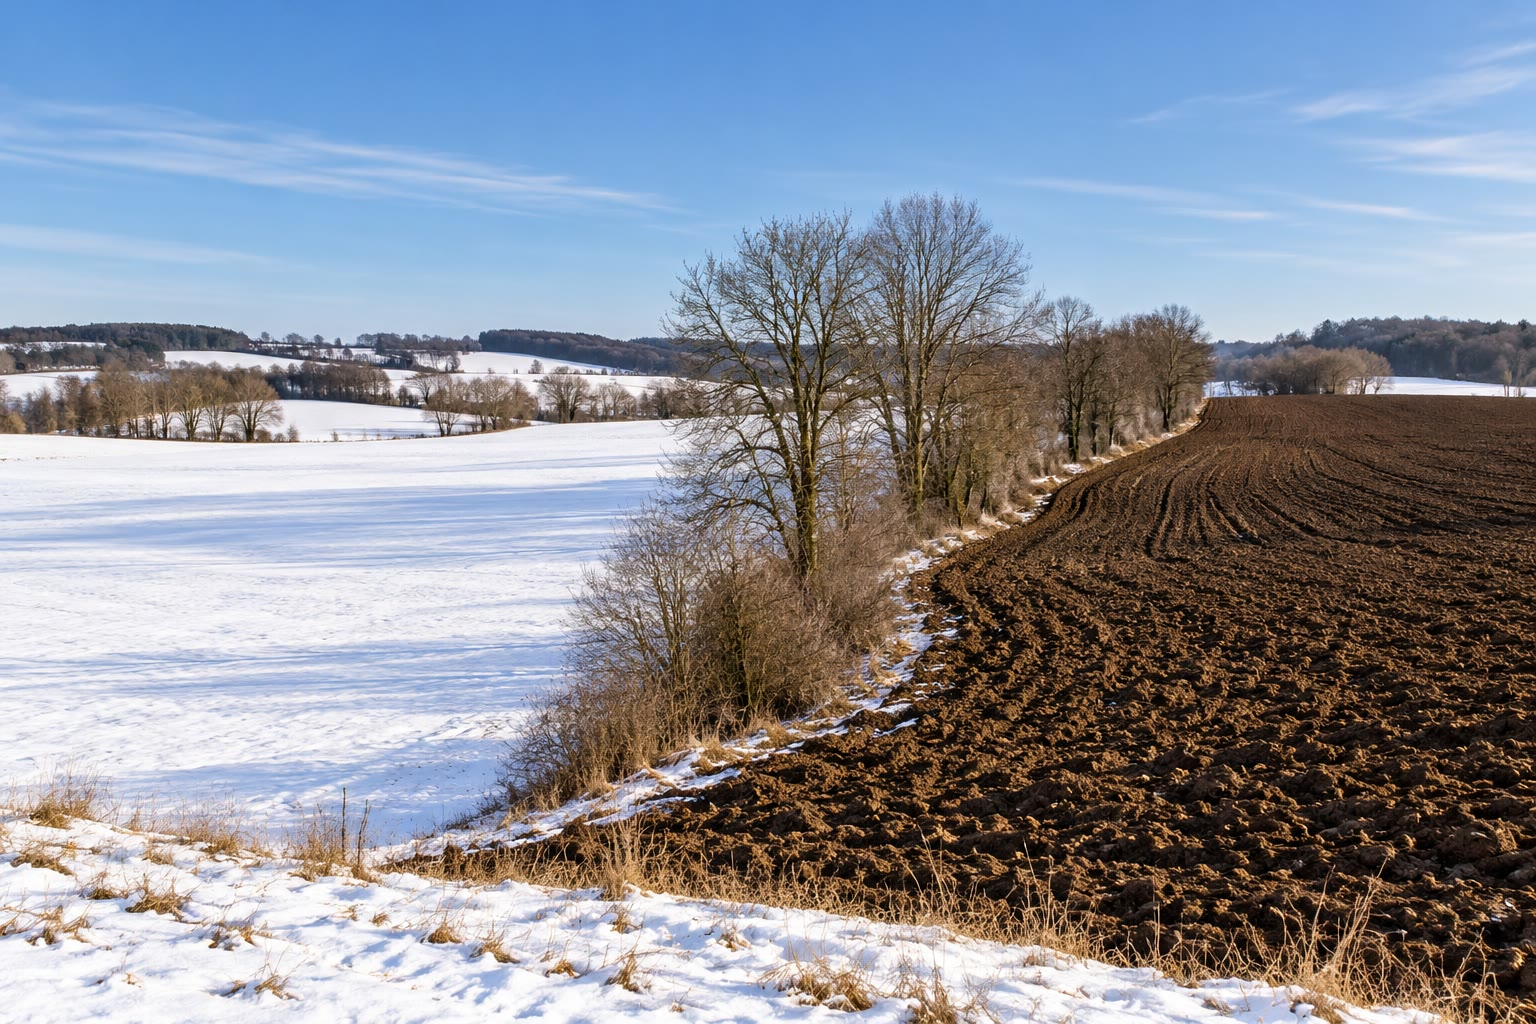
\includegraphics[width=0.7\linewidth]{images/book2/ai/g10-snow-and-ploughed-field.jpg}

{\small Een winterochtend na een paar zonnige dagen: de sneeuw ligt nog op de
wei, maar op de donkere geploegde akker, die veel meer zonlicht absorbeert, is
ze gesmolten.}
\end{omfigure}

Voor de Aarde als geheel meten satellieten het naar de ruimte weerkaatste
zonlicht rechtstreeks: gemiddeld \qty{100}{W/m^2} van de \qty{340}{W/m^2} die
aankomen, een \omterm{def:g10:earth-energy-budget:albedo}{albedo} van $100/340 \approx 0.29$. Wolken zijn de belangrijkste
weerkaatsers: dezelfde metingen, met de wolken er rekenkundig uit gehaald, geven
maar \qty{53}{W/m^2} weerkaatst.
% ledger: ipcc:budget-toa, ipcc:budget-clearsky, earth:albedo

\begin{example}[Het zonlicht dat de Aarde absorbeert]\label{ex:g10:earth-energy-budget:absorbed}
% ledger: earth:TSI, earth:albedo, earth:Rmean (computed in figdata/grade-10/energy_budget.py)
Met een bondalbedo van 0.294 absorbeert elke vierkante meter gemiddeld $340
\times (1 - 0.294) \approx \qty{240}{W/m^2}$. Over de hele bol, met oppervlakte
$4\pi R^2 = 4\pi \times (\qty{6.371e6}{m})^2 \approx \qty{5.10e14}{m^2}$,
absorbeert de Aarde $240 \times 5.10\times10^{14} \approx \qty{1.22e17}{W}$
zonlicht: dit vermogen drijft de winden, de zeestromingen en de waterkringloop
aan.
\end{example}

\section{De wereldwijde energiebalans}

Waar gaan die \qty{240}{W/m^2} naartoe? Metingen van satellieten, van
instrumenten op de grond en van schepen, gecombineerd met modellen van de
atmosfeer, geven vandaag een samenhangend antwoord, gemiddeld over de wereld en
over meerdere jaren. Het wetenschappelijke evaluatierapport van 2021 vat het
samen in het diagram hieronder, en stelt dat de wereldgemiddelde componenten
nu nauwkeuriger bekend zijn, aan de top van de atmosfeer en aan het oppervlak
(\emph{hoge betrouwbaarheid}).
% ledger: ipcc:budget-confidence

\begin{definition}[Energiebalans]\label{def:g10:earth-energy-budget:energy-budget}
De \emph{energiebalans}\index{energiebalans} van een systeem --- de hele Aarde,
haar oppervlak of haar atmosfeer --- is de boekhouding van alle energie die
erin komt en eruit gaat, waarbij elke stroom wordt gegeven als een gemiddeld
vermogen per vierkante meter aardoppervlak. De balans is \emph{sluitend} als wat
erin komt gelijk is aan wat eruit gaat; anders wint of verliest het systeem
energie en warmt het op of koelt het af.
\end{definition}

Het oppervlak verliest ook energie zonder straling: water verdampt uit de zee en
uit bladeren, en de grond verwarmt de lucht die ermee in contact is.

\begin{definition}[Latente warmte; voelbare warmte]\label{def:g10:earth-energy-budget:latent-heat}
De \emph{latente warmte}\index{latente warmte} van een stof is de energie die
ze opneemt wanneer ze van toestand verandert zonder van temperatuur te
veranderen --- bij smelten of verdampen --- en die ze teruggeeft bij de
omgekeerde overgang. Voor water dat verdampt bij \qty{15}{\degreeCelsius} is
dat ongeveer \qty{2.47}{MJ} per kilogram. In de \omterm{def:g10:earth-energy-budget:energy-budget}{energiebalans} is de
\emph{latentewarmtestroom} de energie die verdamping aan het oppervlak onttrekt
en die de waterdamp in de lucht vrijgeeft waar hij tot wolken condenseert. De
stroom van \emph{voelbare warmte}\index{voelbare warmte} is de energie die het
oppervlak doorgeeft aan de lucht die ermee in contact is, waardoor die lucht
opwarmt, en die opstijgende lucht naar boven voert.
\end{definition}
% ledger: nist:water-latent

\begin{omfigure}
\begin{tikzpicture}[font=\footnotesize, >={Stealth[length=2.2mm, width=2mm]}, line width=1.4pt]
  % layers
  \fill[omDef!8] (0,0.5) rectangle (12.8,4.5);
  \fill[omExo!35] (0,0) rectangle (12.8,0.5);
  \draw[thin, black!60] (0,0.5) -- (12.8,0.5);
  \draw[thin, black!60, dashed] (0,4.5) -- (12.8,4.5);
  \node[anchor=east, black!70, align=right] at (-0.1,5.4) {ruimte};
  \node[anchor=east, black!70, align=right] at (-0.1,4.5) {top van de\\atmosfeer};
  \node[anchor=east, black!70, align=right] at (-0.1,2.5) {atmosfeer};
  \node[anchor=east, black!70, align=right] at (-0.1,0.25) {oppervlak};
  \pic[scale=0.7, transform shape] at (4.3,3.0) {puffycloud};
  \pic[scale=0.7, transform shape] at (6.2,3.0) {puffycloud};
  % sunlight
  \draw[->, omProp!90!black] (1.0,6.1) -- (1.0,0.52);
  \draw[->, omProp!90!black] (1.0,3.0) -- (1.6,3.0);
  \node[anchor=west, align=left] at (1.65,3.0) {80 geabsorbeerd\\door de lucht};
  \node[anchor=west] at (1.05,1.3) {185};
  \draw[->, omProp!55] (4.3,3.7) -- (4.3,6.1);
  \node[anchor=east] at (4.25,5.0) {75};
  \draw[->, omProp!55] (5.25,0.52) -- (5.25,6.1);
  \node[anchor=west] at (5.3,1.2) {25};
  % heat
  \draw[->, omMeth!80!black] (6.2,0.52) -- (6.2,2.95);
  \draw[->, omMeth!80!black] (7.8,0.52) -- (7.8,2.0);
  % infrared
  \draw[->, omThm!80!black] (9.2,0.52) -- (9.2,4.0);
  \draw[->, omThm!80!black] (10.7,3.4) -- (10.7,6.1);
  \draw[->, omThm!50] (12.1,4.0) -- (12.1,0.52);
  % words above the top of the atmosphere
  \node[anchor=south, align=center] at (1.0,6.15) {340\\inkomend};
  \node[anchor=south, align=center] at (4.78,6.15) {100\\weerkaatst};
  \node[anchor=south, align=center] at (7.7,5.0) {onbalans\\$+0.7$ geabsorbeerd};
  \node[anchor=south, align=center] at (10.7,6.15) {239 infrarood\\naar de ruimte};
  % words below the surface
  \node[anchor=north, align=center] at (1.0,-0.05) {160\\geabsorbeerd};
  \node[anchor=north, align=center] at (6.2,-0.05) {82\\latente\\warmte};
  \node[anchor=north, align=center] at (7.8,-0.05) {21\\voelbare\\warmte};
  \node[anchor=north, align=center] at (9.4,-0.05) {398\\uitgezonden};
  \node[anchor=north, align=center] at (12.1,-0.05) {342\\tegen-\\straling};
\end{tikzpicture}

{\small De wereldgemiddelde \omterm{def:g10:earth-energy-budget:energy-budget}{energiebalans} van de Aarde aan het begin van de
21e eeuw, in \unit{W/m^2} gemiddeld over het hele oppervlak. Oranje: zonlicht;
groen: warmte die door verdamping en door warme lucht wordt meegevoerd; rood:
infrarood. Van de 100 weerkaatste komen er 25 van het oppervlak en 75 van
wolken, de lucht en het stof erin. Het infrarood naar de ruimte omvat het deel
van de uitstraling van het oppervlak dat recht door de lucht ontsnapt.
Gegevens: IPCC, zesde evaluatierapport, werkgroep~I, figuur~7.2.}
\end{omfigure}
% ledger: ipcc:budget-toa, ipcc:budget-surface

\begin{method}[Een energiebalansdiagram lezen]\label{met:g10:earth-energy-budget:reading}
\begin{enumerate}
  \item Kies het systeem: de hele Aarde (een lijn boven de atmosfeer), het
        oppervlak, of de atmosfeer (de laag ertussen).
  \item Som de pijlen op die erin gaan en tel ze op; som de pijlen op die
        eruit gaan en tel ze op.
  \item Vergelijk de twee sommen. Zijn ze gelijk binnen de afronding van de
        getallen, dan is het systeem in evenwicht; het verschil is wat het per
        seconde en per vierkante meter wint (of verliest).
\end{enumerate}
\end{method}

\begin{proposition}[De balans sluit]\label{prop:g10:earth-energy-budget:balance}
Binnen de afronding van de getallen sluit de balans in het diagram hierboven
voor de Aarde als geheel, voor het oppervlak en voor de atmosfeer, op een klein
overschot na van ongeveer \qty{0.7}{W/m^2} dat de Aarde absorbeert en niet
teruggeeft.
\end{proposition}

\begin{proof}
\emph{Hele Aarde:} erin 340; eruit $100 + 239 = 339$. \emph{Oppervlak:} erin
$160 + 342 = 502$; eruit $82 + 21 + 398 = 501$. In beide gevallen is het
overschot, ongeveer 1, de afgeronde onbalans van 0.7. \emph{Atmosfeer:} noem $W$
het deel van het infrarood van het oppervlak dat door de lucht naar de ruimte
ontsnapt. De lucht ontvangt $80 + 82 + 21 + (398 - W) = 581 - W$ en zendt
$342$ naar beneden en $239 - W$ naar boven uit, samen $581 - W$: in evenwicht,
wat $W$ ook is.
\end{proof}
% ledger: ipcc:budget-toa, ipcc:budget-surface (closures checked in figdata/grade-10/energy_budget.py)

Het diagram toont ook het broeikaseffect aan het werk. Het oppervlak ontvangt
van de lucht \qty{342}{W/m^2} als infrarood --- meer dan twee keer het zonlicht
dat het absorbeert, \qty{160}{W/m^2}. Daardoor kan het \qty{398}{W/m^2}
uitzenden, de uitstraling van een lichaam van ongeveer \qty{15}{\degreeCelsius},
terwijl de Aarde maar \qty{239}{W/m^2} naar de ruimte stuurt. De
natuurkundeboeken bouwen het model dat deze getallen met de temperatuur
verbindt; dit boek gebruikt de gemeten stromen.

\begin{example}[Een meter water per jaar]\label{ex:g10:earth-energy-budget:evaporation}
% ledger: ipcc:budget-surface, nist:water-latent (computed in figdata/grade-10/energy_budget.py)
De latentewarmtestroom, \qty{82}{W/m^2}, verdampt elke seconde $82/2.47\times
10^6 \approx \qty{3.3e-5}{kg}$ water per vierkante meter. Over een jaar,
$3.16\times10^7$ seconden, is dat ongeveer \qty{1050}{kg}, een laag water van
\qty{1.05}{m} dik over de hele Aarde. De lucht bevat telkens maar een beetje
water, dus vrijwel alles valt terug als regen en sneeuw: de latentewarmtestroom
en de jaarlijkse neerslag van de planeet zijn twee kanten van dezelfde
waterkringloop.
\end{example}

\begin{remark}[De onbalans]\label{rem:g10:earth-energy-budget:imbalance}
% ledger: ipcc:budget-toa, ipcc:heating
Het overschot van \qty{0.7}{W/m^2} lijkt piepklein naast stromen van honderden
watt, maar over de hele Aarde is het $0.7 \times 5.10\times10^{14} \approx
\qty{3.6e14}{W}$, grotendeels opgeslagen in de oceaan, die opwarmt. Het is geen
natuurconstante: het is de laatste decennia gegroeid, zoals
\cref{ch:g12:climate-change} uitlegt.
\end{remark}

\section{Overschot en tekort}

De balans sluit voor de Aarde als geheel, maar niet op elke breedte.

\begin{omfigure}
\begin{tikzpicture}
\begin{axis}[omrecord, width=0.86\linewidth, height=5.6cm, xmin=0, xmax=90,
  ymin=0, ymax=450, xlabel={breedte (\unit{\degree})},
  ylabel={jaargemiddelde instraling (\unit{W/m^2})}, xtick={0,15,...,90},
  tick label style={font=\small}, label style={font=\small}]
\addplot[omThm!85!black, thick] table[x=lat, y=Qann] {figdata/out/grade-10-energy_budget-annual.dat};
\addplot[omDef!80!black, dashed, domain=0:90] {340.25};
\node[anchor=south west, font=\footnotesize, omDef!80!black] at (axis cs:2,343) {wereldgemiddelde, 340};
\node[anchor=south west, font=\footnotesize, omThm!85!black] at (axis cs:62,232) {jaargemiddelde};
\end{axis}
\end{tikzpicture}

{\small Jaargemiddelde \omterm{def:g10:earth-energy-budget:insolation}{instraling} aan de top van de atmosfeer tegen de breedte
(op beide halfronden dezelfde; berekend uit de zonneconstante en de helling van
de as). Tussen de evenaar en ongeveer \qty{37}{\degree} ligt ze boven het
wereldgemiddelde; dichter bij de polen blijft ze eronder.}
\end{omfigure}

De tropen absorberen veel meer zonlicht dan de poolgebieden, en hun lage \omterm{def:g10:earth-energy-budget:albedo}{albedo}
vergroot het verschil nog. Het infrarood dat ze naar de ruimte sturen is ook
groter, omdat ze warmer zijn, maar het varieert veel minder met de breedte.
Daardoor absorberen de gebieden rond de evenaar gemiddeld ongeveer
\qty{200}{W/m^2} meer dan ze weerkaatsen en uitstralen, en stralen de gebieden
bij de polen ongeveer \qty{200}{W/m^2} meer uit dan ze absorberen.
% ledger: nasaeo:surplus

\begin{definition}[Warmtetransport naar de polen]\label{def:g10:earth-energy-budget:heat-transport}
Het \emph{warmtetransport naar de polen}\index{warmtetransport naar de polen}
is de energiestroom die de bewegingen van de atmosfeer en van de oceaan van de
tropen naar de polen voeren. Het wordt gemeten door een breedtecirkel heen, in
petawatt (\qty{1}{PW} = \qty{e15}{W}).
\end{definition}

Zonder dat transport zouden de tropen steeds heter en de polen steeds kouder
worden, tot elke breedte haar eigen balans sloot. De atmosfeer doet het meeste
werk: warme lucht die naar de polen stroomt en koude lucht die naar de evenaar
terugkeert, en waterdamp die zijn \omterm{def:g10:earth-energy-budget:latent-heat}{latente warmte} ver van de plaats waar hij
verdampte vrijgeeft. De zeestromingen voeren de rest. Schattingen op basis van
metingen geven voor het transport door de atmosfeer een maximum van ongeveer
\qty{5.0}{PW} bij \qty{43}{\degree} NB, met vergelijkbare waarden bij
\qty{40}{\degree} ZB; de oceaan voert alleen dicht bij de evenaar meer dan de
atmosfeer, tussen \qty{0}{\degree} en \qty{17}{\degree} NB, en op
\qty{35}{\degree} NB, waar het totale transport het grootst is, neemt de
atmosfeer er \qty{78}{\percent} van voor haar rekening. Het totaal is daar het
grootst omdat \qty{35}{\degree} ongeveer de breedte is waar het overschot
overgaat in het tekort: naar de evenaar toe blijft het transport het overschot
van elke breedte die het passeert verzamelen; naar de pool toe put elke breedte
eruit.
% ledger: trenberth:transport

\begin{omfigure}
\begin{tikzpicture}[font=\footnotesize, >={Stealth[length=2mm]}]
  \def\R{2.4}
  \begin{scope}
    \clip (0,0) circle (\R);
    \fill[omThm!22] (-\R,{-\R*sin(35)}) rectangle (\R,{\R*sin(35)});
    \fill[omDef!22] (-\R,{\R*sin(35)}) rectangle (\R,\R);
    \fill[omDef!22] (-\R,-\R) rectangle (\R,{-\R*sin(35)});
  \end{scope}
  \draw[thick] (0,0) circle (\R);
  \draw[black!50] (-\R,0) -- (\R,0);
  \foreach \s in {1,-1} \draw[black!40, dashed] ({-\R*cos(35)},{\s*\R*sin(35)}) -- ({\R*cos(35)},{\s*\R*sin(35)});
  \node at (0,0.45) {overschot};
  \node at (0,1.95) {tekort};
  \node at (0,-1.95) {tekort};
  \node[anchor=west, black!60] at (\R+0.05,0) {evenaar};
  \node[anchor=west, black!60] at ({\R*cos(35)+0.05},{\R*sin(35)}) {\qty{35}{\degree} NB};
  \node[anchor=west, black!60] at ({\R*cos(35)+0.05},{-\R*sin(35)}) {\qty{35}{\degree} ZB};
  \foreach \s in {1,-1} {
    \draw[->, very thick, omProp!90!black] ({-(\R+0.35)*cos(10)},{\s*(\R+0.35)*sin(10)}) arc ({180-10*\s}:{180-70*\s}:{\R+0.35});
    \draw[->, thick, omMeth!80!black] ({-(\R-0.45)*cos(8)},{\s*(\R-0.45)*sin(8)}) arc ({180-8*\s}:{180-55*\s}:{\R-0.45});
  }
  \node[anchor=east, omProp!90!black, align=right] at (-\R-0.75,1.6) {atmosfeer};
  \node[anchor=east, omProp!90!black, align=right] at (-\R-0.75,-1.6) {atmosfeer};
  \node[omMeth!80!black] at (-1.25,0.62) {oceaan};
  \node[omMeth!80!black] at (-1.25,-0.62) {oceaan};
\end{tikzpicture}

{\small Tussen ongeveer \qty{35}{\degree} ZB en \qty{35}{\degree} NB absorbeert
de Aarde meer energie dan ze uitstraalt; dichter bij de polen straalt ze meer uit
dan ze absorbeert. De atmosfeer (oranje) en de oceaan (groen) voeren het
overschot naar de polen. Schematisch: de breedte van de pijlen is niet op
schaal.}
\end{omfigure}

Dit transport is de motor van het weer. De convectiecellen en de wereldwijde
winden van Boek 1, de stormen van \cref{ch:g10:storms-and-cyclones} en de grote
zeestromingen van \cref{ch:g10:layered-ocean} verplaatsen allemaal warmte van
waar de Zon te veel geeft naar waar ze te weinig geeft.

\section{Waar de energie blijft}

Bijna alle energie van het zonlicht die de Aarde absorbeert, eindigt als warmte:
ze verwarmt de grond, de zee en de lucht, verdampt water, drijft de winden en
de stromingen aan, en vertrekt weer als infrarood licht. Een piepklein deel
volgt een andere weg: fotosynthese slaat het op in de chemische bindingen van
suikers, en van daaruit in alle levende materie van de planeet.

\begin{example}[Het aandeel van de fotosynthese]\label{ex:g10:earth-energy-budget:photosynthesis}
% ledger: field:npp, nist:glucose-combustion, earth:Rmean (computed in figdata/grade-10/energy_budget.py)
Planten op het land en algen in de zee slaan, na hun eigen behoeften, elk jaar
ongeveer \num{105} miljard ton koolstof op in nieuwe levende materie, ruwweg de
helft op het land en de helft in de oceaan: ecologen noemen dat de netto
primaire productie van de planeet. De verbranding van een mol glucose,
\ce{C6H12O6}, die zes mol koolstof bevat, \qty{72}{g}, levert
\qty{2805}{kJ}: ongeveer \qty{38.9}{kJ} per gram koolstof. De energie die elk
jaar wordt opgeslagen, is $1.049\times10^{17}\,\unit{g} \times \qty{38.9e3}{J/g} \approx
\qty{4.1e21}{J}$, een vermogen van $4.1\times10^{21}/3.16\times10^{7} \approx
\qty{1.3e14}{W}$. Vergeleken met de \qty{1.22e17}{W} zonlicht die de Aarde
absorbeert, is dat ongeveer \qty{0.1}{\percent}.
\end{example}

\begin{remark}[Een klein aandeel, een grote rol]\label{rem:g10:earth-energy-budget:life}
Een duizendste van het geabsorbeerde zonlicht voedt bijna al het leven op
Aarde, en de resten van planten en algen die honderden miljoenen jaren lang zijn
begraven, vormen steenkool, aardolie en aardgas
(\cref{ch:g11:fossil-fuel-geology}). De rest van het zonlicht --- meer dan
99.9 procent --- houdt de planeet warm en haar lucht, water en weer in beweging.
\end{remark}

\section{Oefeningen}

\begin{exercise}[$\star$]\label{exo:g10:earth-energy-budget:1}
Definieer de \omterm{def:g10:earth-energy-budget:insolation}{instraling} van een plaats en het \omterm{def:g10:earth-energy-budget:albedo}{albedo} van een oppervlak. Wat
weerkaatst het grootste deel van het zonlicht, verse sneeuw of de open oceaan?
\end{exercise}

\begin{exercise}[$\star$]\label{exo:g10:earth-energy-budget:2}
Geef met behulp van het energiebalansdiagram van dit hoofdstuk, als percentage
van de \qty{340}{W/m^2} die aan de top van de atmosfeer aankomen, het deel dat
naar de ruimte wordt weerkaatst, het deel dat de lucht absorbeert en het deel
dat het oppervlak absorbeert.
\end{exercise}

\begin{exercise}[$\star$]\label{exo:g10:earth-energy-budget:3}
Een zomerzon levert \qty{800}{W/m^2} op de grond. Hoeveel vermogen absorbeert
een vierkante meter die met vers asfalt (\omterm{def:g10:earth-energy-budget:albedo}{albedo} 0.04) is bedekt, en een die met
verse sneeuw (\omterm{def:g10:earth-energy-budget:albedo}{albedo} 0.85) is bedekt?
\end{exercise}

\begin{exercise}[$\star$]\label{exo:g10:earth-energy-budget:4}
Wat voert meer energie weg van het aardoppervlak: verdamping of het opwarmen van
de lucht die met de grond in contact is? Beschrijf in twee zinnen hoe de energie
die verdamping aan de zee onttrekt, de lucht hoog erboven bereikt.
\end{exercise}

\begin{exercise}[$\star$]\label{exo:g10:earth-energy-budget:5}
Leg uit waarom de daggemiddelde \omterm{def:g10:earth-energy-budget:insolation}{instraling} op de Noordpool in december nul is,
en geef de breedte waarboven dat bij de decemberzonnewende gebeurt.
\end{exercise}

\begin{exercise}[$\star\star$]\label{exo:g10:earth-energy-budget:6}
Bereken met \cref{prop:g10:earth-energy-budget:height} het vermogen dat een
horizontale vierkante meter aan de top van de atmosfeer ontvangt wanneer de Zon
\qty{90}{\degree}, \qty{30}{\degree} en \qty{10}{\degree} boven de horizon staat.
Op welke hoogte van de Zon ontvangt de vierkante meter de helft van $S_0$?
\end{exercise}

\begin{exercise}[$\star\star$]\label{exo:g10:earth-energy-budget:7}
Controleer volgens \cref{met:g10:earth-energy-budget:reading} de balans van het
zonlicht alleen: hoeveel van de \qty{340}{W/m^2} die aankomen, wordt
weerkaatst, door de lucht geabsorbeerd en door het oppervlak geabsorbeerd? Is
de som van de drie 340? Controleer ook dat het zonlicht dat het oppervlak
bereikt, \qty{185}{W/m^2}, daar wordt weerkaatst of geabsorbeerd.
\end{exercise}

\begin{exercise}[$\star\star$]\label{exo:g10:earth-energy-budget:8}
Bereken met de gemiddelde straal van de Aarde, \qty{6371}{km}, de oppervlakte
van de schijf die het zonlicht opvangt en het vermogen dat ze opvangt, en daarna
de oppervlakte van de bol. Leid daaruit het gemiddelde vermogen per vierkante
meter van de bol af.
\end{exercise}

\begin{exercise}[$\star\star$]\label{exo:g10:earth-energy-budget:9}
Het overschot van de Aarde is \qty{0.7}{W/m^2} over een oppervlakte van
\qty{5.10e14}{m^2}. Hoeveel energie, in joule, wint de Aarde in een jaar van
$3.16\times10^7$ seconden?
\end{exercise}

\begin{exercise}[$\star\star$]\label{exo:g10:earth-energy-budget:10}
Met de wolken er rekenkundig uit gehaald, zou de Aarde \qty{53}{W/m^2}
weerkaatsen in plaats van \qty{100}{W/m^2}, en \qty{267}{W/m^2} infrarood naar
de ruimte sturen in plaats van \qty{239}{W/m^2}. Hoeveel veranderen de wolken
het geabsorbeerde zonlicht, en het verloren infrarood? Warmen de wolken de Aarde
per saldo op, of koelen ze haar af?
\end{exercise}

\begin{exercise}[$\star\star$]\label{exo:g10:earth-energy-budget:11}
Lees de krommen van de daggemiddelde \omterm{def:g10:earth-energy-budget:insolation}{instraling} in dit hoofdstuk af. In welke
maanden is de daggemiddelde \omterm{def:g10:earth-energy-budget:insolation}{instraling} op de Noordpool groter dan op de evenaar?
Waarom vertoont de kromme van de evenaar twee maxima en niet één?
\end{exercise}

\begin{exercise}[$\star\star\star$]\label{exo:g10:earth-energy-budget:12}
De latente verdampingswarmte van water is \qty{2.47}{MJ/kg} en de
latentewarmtestroom \qty{82}{W/m^2}. Bereken de dikte van de laag water, in
millimeter, die elke dag van de gemiddelde vierkante meter van de Aarde
verdampt, en in meter per jaar (een liter water, uitgespreid over een vierkante
meter, geeft een laag van \qty{1}{mm} dik).
\end{exercise}

\begin{exercise}[$\star\star\star$]\label{exo:g10:earth-energy-budget:13}
Op de Noordpool draait de Zon rond aan de hemel op een hoogte gelijk aan haar
declinatie $\delta$, dus de daggemiddelde \omterm{def:g10:earth-energy-budget:insolation}{instraling} is daar $S_0 \sin
\delta$. Zoek de declinatie waarbij de pool gemiddeld over de dag evenveel
ontvangt als de evenaar bij een equinox, $S_0/\pi$. Voor de declinatie geldt
$\sin\delta = \sin 23.44^\circ \times \sin\lambda$, waarbij de hoek $\lambda$
in een jaar gelijkmatig met \qty{360}{\degree} toeneemt, vanaf
\qty{0}{\degree} bij de maartequinox (\qty{90}{\degree} bij de
junizonnewende). Gedurende ongeveer hoeveel dagen per jaar ontvangt de pool meer
dan $S_0/\pi$?
\end{exercise}

\begin{exercise}[$\star\star\star$]\label{exo:g10:earth-energy-budget:14}
Stel dat in de zomer een oppervlakte van \qty{1e12}{m^2} zee-ijs (\omterm{def:g10:earth-energy-budget:albedo}{albedo} 0.6)
smelt en wordt vervangen door open oceaan (\omterm{def:g10:earth-energy-budget:albedo}{albedo} 0.06), onder zonlicht van
gemiddeld \qty{300}{W/m^2} aan het oppervlak. Bereken het extra geabsorbeerde
vermogen. Vergelijk het met het vermogen dat alle fotosynthese op Aarde
opslaat, \qty{1.3e14}{W}, en leg uit waarom deze wisseling van oppervlakken
zichzelf versterkt.
\end{exercise}

\begin{exercise}[$\star\star\star$]\label{exo:g10:earth-energy-budget:15}
De afstand van de Aarde tot de Zon is \num{147.1} miljoen kilometer op het
dichtstbijzijnde punt en \num{152.1} miljoen op het verste, met een gemiddelde
van \num{149.6} miljoen, waar $S_0 = \qty{1361}{W/m^2}$. Bereken de
bestralingssterkte van de Zon bij de twee uitersten. Het verschil is bijna
\qty{90}{W/m^2}; op \qty{60}{\degree} NB is de daggemiddelde \omterm{def:g10:earth-energy-budget:insolation}{instraling} ongeveer
\qty{490}{W/m^2} in juni en \qty{24}{W/m^2} in december. Leg uit waarom de
afstand niet de oorzaak van de seizoenen kan zijn.
\end{exercise}

\section{Probleem: een zonnestraal volgen}

\begin{problem}[{Weekendprobleem --- van het zonlicht dat de Aarde bereikt tot
het deel dat het leven opslaat}]
\label{pb:g10:earth-energy-budget:1}
% ledger: earth:TSI, earth:Rmean, ipcc:budget-toa, ipcc:budget-surface, ipcc:budget-clearsky, nist:water-latent, field:npp, nist:glucose-combustion (all results computed in figdata/grade-10/energy_budget.py or from the rounded data below)
Gebruik $S_0 = \qty{1361}{W/m^2}$, de straal van de Aarde $R = \qty{6371}{km}$,
$\sigma = \qty{5.67e-8}{W.m^{-2}.K^{-4}}$, een jaar van $3.156\times10^7$
seconden, de stromen van het energiebalansdiagram, een latente
verdampingswarmte van \qty{2.47}{MJ/kg}, een wereldwijde netto primaire productie
van \num{104.9} miljard ton koolstof per jaar, en \qty{2805}{kJ} die vrijkomt
bij de verbranding van een mol glucose (\qty{72.07}{g} koolstof).

\medskip
\noindent\textbf{Deel I --- De meetkunde van het zonlicht.}
\begin{enumerate}
  \item Bereken de oppervlakte van de schijf die het zonlicht opvangt, $\pi R^2$,
        in vierkante meter.
  \item Bereken het vermogen aan zonlicht dat ze opvangt.
  \item Bereken de oppervlakte van het aardoppervlak, $4\pi R^2$.
  \item Leid daaruit het gemiddelde vermogen af dat per vierkante meter aan de
        top van de atmosfeer aankomt.
  \item Bij een equinox staat de Zon om 12 uur 's middags in het zenit boven de
        evenaar en \qty{30}{\degree} boven de horizon op \qty{60}{\degree} NB. Wat
        ontvangt een horizontale vierkante meter op elk van beide plaatsen?
\end{enumerate}

\medskip
\noindent\textbf{Deel II --- Albedo.}
\begin{enumerate}[resume]
  \item Bereken uit de \qty{100}{W/m^2} die worden weerkaatst het \omterm{def:g10:earth-energy-budget:albedo}{albedo} van de Aarde.
  \item Bereken het geabsorbeerde vermogen per vierkante meter en voor de hele Aarde.
  \item Zonder wolken zou \qty{53}{W/m^2} worden weerkaatst. Hoe groot zou het
        \omterm{def:g10:earth-energy-budget:albedo}{albedo} dan zijn? Met welke factor verhogen wolken het?
  \item Bereken de \omterm{def:g10:habitable-planet:equilibrium-temperature}{evenwichtstemperatuur} die hoort bij het geabsorbeerde
        vermogen van vraag 7 (\cref{ch:g10:habitable-planet}), en vergelijk die
        met de \qty{288}{K} van het oppervlak.
\end{enumerate}

\medskip
\noindent\textbf{Deel III --- Het oppervlak.}
\begin{enumerate}[resume]
  \item Tel de energiestromen op die het oppervlak binnenkomen.
  \item Tel de stromen op die het verlaten, en vergelijk.
  \item Hoeveel keer groter dan het zonlicht dat het oppervlak absorbeert, is het
        infrarood dat het van de lucht ontvangt? Wat laat dat zien?
  \item Bereken de massa water die in een jaar van een vierkante meter verdampt,
        en de dikte van de laag die ze vormt.
  \item Bereken het totale vermogen van de onbalans, \qty{0.7}{W/m^2}, over de
        hele Aarde.
\end{enumerate}

\medskip
\noindent\textbf{Deel IV --- Het aandeel van het leven.}
\begin{enumerate}[resume]
  \item Bereken de energie die per gram in glucose vastgelegde koolstof wordt opgeslagen.
  \item Bereken de energie die de netto primaire productie in een jaar opslaat.
  \item Reken die om naar een vermogen.
  \item Druk het uit per vierkante meter aardoppervlak.
  \item Vergelijk het met de onbalans van vraag 14.
  \item Welk deel van het door de Aarde geabsorbeerde zonlicht (vraag 7) slaat
        fotosynthese op?
\end{enumerate}
\end{problem}
